% This infolevnull section is just for the ESAD.  We should try to
% merge it with the text.  The infolevnull section applies
% to both SHMS and HMS chambers
\infoleveqnull{
\section{Drift Chambers}
The Drift Chambers in the HMS and SHMS spectrometers
provide a
precise ($\pm 125~\mu$m) measurement of the position and angle of
incidence of particles at the respective spectrometer focal planes.
This
information may be combined with the knowledge of the spectrometer
optics to determine the position and angle of the particles in the
target.

Operation of the Hall C drift chambers requires the application of both High Voltage
(HV) across the chambers themselves and Low Voltage (LV) across the
preamplifier/discriminator cards, which are mounted on the sides of
the drift chabmers.
The chamber gas is a combination of argon (Ar) and flammable ethane
(C$_2$H$_6$) which is bubbled through alcohol.  Gas is routed from
bottles located next to the Hall C gas shed, through the gas mixing
system in the gas shed, to the chambers in the spectrometer detector
huts.

\subsection{Hazards}

The following hazards are associated with the chambers:

\begin{description}
\item {\bf The High Voltage System}
CAEN SY403 high voltage/low current power supplies provide high
voltages to the chambers in the range of -1.5 kV to -2.5 kV.
\item{\bf Explosive Gas} The Ar~C$_2$H$_6$ chamber gas is explosive
and must be handled accordingly.  Further, gas flow should be maintained
for at least 24 hours prior to the enabling of HV.
\item{\bf High Pressure Gas Bottles} The gas used in the chambers
is supplied in high pressure ($\ge$ 2000 psi) gas bottles. This
confined high pressure gas represents a tremendous (potentially lethal)
amount of stored energy.
\end{description}


\subsection{Mitigations}

For the HV, red HV RG-59/U cables good to 5 kV with standard SHV
connectors are used to connect the power supply to the chamber
high voltage distribution splitters on each chamber.
A given chamber draws a current
from  50--100 nA.  When servicing the chambers, the HV for that
element must be turned off and disconnected.

The high pressure gas bottles are stored far from the equipment in
a controlled
area as discussed in the Hall C gas handling section of the
operations manual.


\subsection{Responsible Personnel}

The individuals responsible for the operation
of the drift chambers are shown in Table \ref{tab:dc:personnel}.

\begin{namestab}{tab:dc:personnel}{DC responsible personnel}{%
      DC responsible personnel.}
  \EricChristy{}
  \LiguangTang{}
  \BradSawatzky{}
  \StephenWood{}
%  \MahlonLong{}
  \JoeBeaufait{}
  \JackSegal{}
\end{namestab}

}


\infolevone{
% Details needed
% Location of Acopian supplies - Nominal current draws
% Location/method of threshold control


\subsection{Drift Chambers}
\label{sec:shmschambers}
The drift chambers provide accurate measurements of particles position
and angles in the detector hut.  This information can be combined with
a knowledge of the spectrometer optics to infer particle momenta and
the angles and positions particles at the target.

\begin{figure}[htb]
\begin{center}
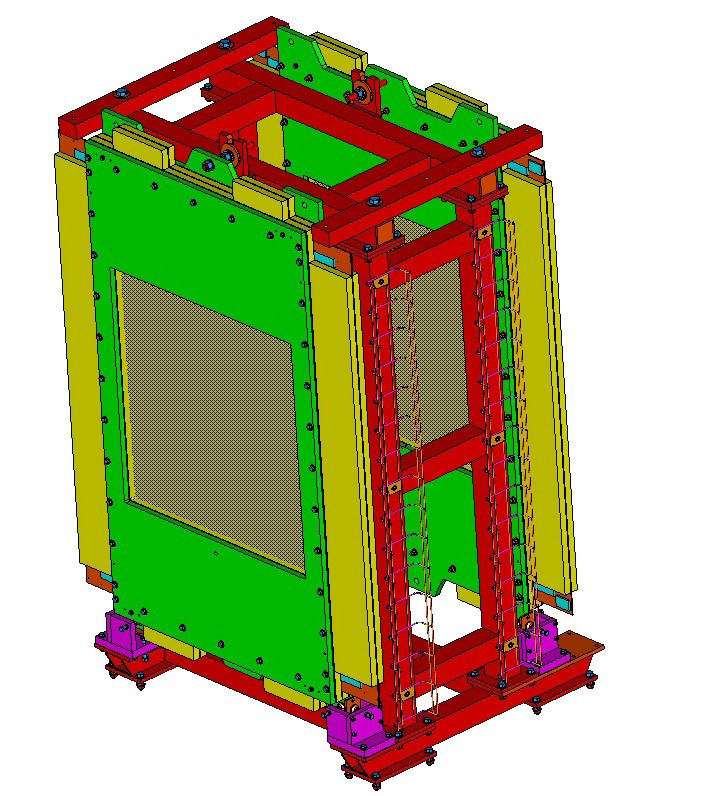
\includegraphics[width=0.75\textwidth]{shms_dcs_frame_drawing.png}
\caption{\label{chamberpair}Technical drawing of the SHMS drift
  chambers mounted in the detector hut frame.}
\end{center}
\end{figure}

The drift chamber package consists of two identical chambers, with 6 planes of
wires each.  (Figure~\ref{chamberpair})  Each wire plane consists of a set of
alternating 20  $\mu\textrm{m}$ gold tungsten sense (anode) wires and 80
$\mu\textrm{m}$ field wires, separated by 0.5cm.  A cathode plane of copper
coated mylar is located between each wire plane, before the first wire plane and
after the last wire plane. In planes labled $X$ and $X^{\prime}$, the wires are
horizontal.  In the $U$ and $U^{\prime}$ planes the wires are rotated
$60^{\circ}$ relative to the $X$ planes while in the $V$ and $V^{\prime}$ planes
the wires are rotated by $-60^{\circ}$.  The
$V^{\prime}$, $X^{\prime}$, and $U^{\prime}$ planes are offset from the unprimed
planes by 0.5 cm.
The first chamber consists of planes
ordered as ($U$, $U^{\prime}$, $X$, $X^{\prime}$, $V^{\prime}$, $V$).  The
second chamber, while of identical design to the first chamber is rotated by
$180^{\circ}$ about the vertical access, so the plane ordering is
($V$, $V^{\prime}$, $X^{\prime}$, $X$, $U^{\prime}$, $U$).  Note however,
this rotation results in the $U$ ($V$) planes in first chamber being parallel
to the $V$ ($U$) planes in the second chamber.
The active area of each chamber is $80~\textrm{cm}\times
80~\textrm{cm}$ which has been set to match the active area for particles in
the SHMS focal plane. Further details about the design and construction of the
drift chambers are in the SHMS Drift Chambers
reference~\cite{howto:shms_drift_chambers}.

The drift chambers 50/50 mixture (by weight) of Ethane/Argon as a
drift gas which
flows across all of the wire planes.  The system that delivers this
gas is described in
\ifdefined\SHMSDCOSP
section 5.1.2 of the Hall C Standard Equipment Manual~\cite{HallCosp}.
\else
section~\ref{sec:chambergas}.
\fi

The high voltage for the SHMS drift chambers is supplied by CAEN
high voltage, low current, power supplies in the electronics room of
the counting
house and can be controlled through a GUI on the console computers.
The operating voltages for the chambers are a nominal -1800V (foil) and -1800V
(potential wires).  Control of the high voltage system is described in
\ifdefined\SHMSDCOSP
section 5.1.1 of the Hall C Standard Equipment Manual~\cite{HallCosp}.
\else
section~\ref{sec:highvoltage}.
\fi

Each anode/sense wire has its own electronic readout through
Nanometrics preamplifier/discriminator cards or LeCroy Corporation LRS
2735DC cards which are interchangeable with the Nanometrics cards.
The discriminator outputs from the cards, each of which instruments 16
sense wires are connected to CAEN V1190 multi-hit TDCs located in the
SHMS electronics hut.
The discriminator cards are powered by +5V and -5V Acopian power
supplies that are
located in the SHMS electronics hut.  The supply currents are several
10s of amps for the positive and negative supplies.
The discriminator thresholds for these cards are controlled by a power
supplies in rack CH03B10 in the Hall C counting house.  Nominal
threshold settings will be posted by on the supply.

\paragraph{Start-of-Run Procedure}
The procedure for turning the chambers on at the start of an
experiment is the following:
\begin{enumerate}
\item Make sure gas is flowing through both chambers.
\item Turn on the low voltage Acopian power supplies in the SHMS detector hut.
\item Turn on the VME crate with the TDCs if it is not already on.
\item Turn on the threshold power supply to the appropriate setting
  (nominally 4V).
\item Turn on the high voltage.
\end{enumerate}

\paragraph{End-of-Run Procedure}
At the end of an experiment or before an extended down, the high
voltage supplies and the Acopian low-voltage supplies should be turned
off.  The ethane gas flow may be shut off, but the argon gas flow
should be left on to keep the chambers clean and dry.

% Add a responsible personell here
}% \infolevone
